\chapter{历史的记录}
% 原书第1页

雍正登位后，与皇三子允祉一起编订了《圣祖仁皇帝庭训格言》，收录了康熙作为父亲平时教育他们时说的话和讲到的往事。其中有一条与天主教传教士徐日昇（Thomas Pereira，1645—1708）相关：


% 原书第1页

\begin{bookquote}朕（注：康熙）虽于谈笑小节，亦必循理。先者，大阿哥管养心殿营造事务时，一日同西洋人徐日昇进内与朕闲谈。中间大阿哥与徐日昇戏曰：“剃汝之须可乎？”徐日昇佯佯不采，云：“欲剃则剃之。”彼时朕即留意大阿哥原是悖乱之人。设曰：“我奏过皇父，剃徐日昇之须。”欲剃则竟剃矣，外国之人谓朕因戏而剃其须，可乎？\end{bookquote}

% 原书第1–2页

\begin{bookquote}其时，朕亦笑曰：“阿哥若欲剃，亦必启奏，然后可剃。”徐日昇一闻朕言，凄然变色，双目含泪，一言不出。既逾数日后，徐日昇独来见朕，涕泣而向朕曰：“皇上何如斯之神也！为皇子者，即剃我外国人之须，有何关系？皇上尚虑及未然，降此谕旨。实令臣难禁受也。”\end{bookquote}

% 原书第2页

\begin{bookquote}厥后四十七年朕不豫时，徐日昇听信外边乱语，以为朕疾难愈，到养心殿大哭，自怨其无造化。随回，至家身故。夫一言可以得人心，而一言亦可以失人心也。\NoteRef{01}{1}\end{bookquote}

% 原书第2页

徐日昇是葡萄牙人，1672年到达澳门，一年后被南怀仁（Ferdinand Verbiest）神父招入宫中，协助观测天文，并教授康熙西方音乐与数学。徐日昇到达北京的1673年，康熙十九岁，而徐日昇二十八岁。这时康熙铲除鳌拜仅过了四年，也就是说，徐日昇在康熙亲政之初就已经来到康熙身边，做了他的老师。徐日昇来到北京时，北京还只有南怀仁、安文思（Gabriel de Magalhaes） 和利类思（Lodovico Buglio）三位神父，因而他也算是出现在康熙身边的第一代神父。在前三位神父相继去世后，徐日昇从1688年开始就成为了康熙身边最为信赖的传教士。也是由于徐日昇入宫时间早，而且西洋传教士在康熙年间归内务府管理，可以进出内廷，因而许多皇子都是徐日昇看着长大的，他们之间也都是老熟人。\NoteRef{01}{2}


% 原书第2–3页

有了这个背景，才能明白上面这段故事中，为什么徐日昇这个外国神父能跟大皇子一起在内廷的养心殿中和康熙闲谈，而大皇子也可以开玩笑说要剪掉徐日昇的大胡子。这段话除了展示徐日昇和康熙一家的亲密关系以外，跟本书有关的内容就是这里提到徐日昇的去世。徐日昇死于1708年12月24日，正是康熙废黜太子以后与朝廷权贵为新太子人选来回争执的时期。这一年，康熙五十四岁。而六十三岁的徐日昇已经行走在康熙身边三十五年了。康熙跟他的儿子们讲起徐日昇生前因为听信外边乱语，以为他生病难愈，而到养心殿大哭，这说明康熙对徐日昇是心存感念的。在感叹康熙与徐日昇的交往之余，对于历史研究来说，这里出现一个问题：为什么平时都能单独见到康熙的徐日昇，这时见不到康熙了，而只能在养心殿大哭？


% 原书第3页

《北京纪事》恰好也记载了徐日昇当时求见康熙而不得的往事，同时还给出了答案。1708年10月17日，康熙在外出狩猎的行程中宣布废黜太子。这个决定，根据传教士的记录并没有和朝中大臣商议。因而康熙在10月底回到北京以后，就拒绝会见任何人，以免有反对废黜太子的人找他。在这个背景下，才有了徐日昇到宫中求见康熙而不得的事。因为康熙担心徐日昇这个老熟人是来给太子求情的。


% 原书第3–4页

为了传教事业，徐日昇等一众传教士几十年来在太子成长的过程中，付出了很多心血。比如早在康熙亲政前，传教士就在康熙的私人圈子中与索额图相识，共同为康熙铲除鳌拜出了力。很多传教士写的记录中都提到过索额图，称他“Sosan （索三）”，因为他是索尼的三儿子。而太子的生母孝诚仁皇后正是索额图大哥的女儿，也就是说，索额图是太子母亲的娘家人。有了索额图这层关系，传教士群体在太子很小的时候，就有机会接近他。


% 原书第4页

尽管1703年索额图因为政治原因倒台去世，传教士群体与太子一系依然维持着联系。1706年，教皇派到中国的使节入京后，除康熙接待之外，太子也专门宴请了他们。教皇使节还乐观地向欧洲汇报过未来中国的皇帝会继续善待天主教。所以，徐日昇等传教士与太子一系交好是康熙很清楚的事，也是当时天下共知的。因而当康熙得知徐日昇来求见时，马上意识到这是来给太子说情，请他三思的。


% 原书第4–5页

据《北京纪事》的主笔纪理安（Kilian Stumpf）神父记载，1708年11月1日，他在宫中看到太监询问来求见康熙的徐日昇，是不是因为听到了什么流言（指废黜太子相关的事）才来的。徐日昇回答，他确实听到了各种流言，但那些他都不关心，也与他无关。他每天过来请安，完全只是担心皇帝的身体被病痛所折磨。太监把徐日昇的话带了进去。过了一会，太监出来传达了康熙的话：“我的身体还好。”《北京纪事》还特地用字母“mini beie (beye) sain”记录下了这个回答，表明当时太监是用满语把康熙的原话传递给徐日昇神父的。\NoteRef{01}{3}这也表明康熙认可徐日昇当时做的是满人传统中奴才对主子的请安。


% 原书第5页

至于为什么康熙要在行营路上宣布废黜太子，而且回京后一段时间内拒不见人，将会在后面的章节中细说。而在使用《北京纪事》来增补清史前，这一章要先简单介绍一下什么是本书所谓的正史，哪些清朝的材料被本书当作了正史。这样可以在本书一开始，明确书名中所谓“正史虚构”是哪里的虚构。其次，在使用传教士的记录前，本书会简要介绍一下北京传教士在当时北京城中的地位，以及为什么这些西洋人有资格知道宫内之事。同时，这一章也会介绍《北京纪事》这份资料的基本情况和特点，说明为什么这是一份可靠的历史资料。


\begin{sectionnotes}

% 原书注释：原书第388页
\BookNote{01}{1}{《圣祖仁皇帝庭训格言》，《景印文渊阁四库全书》，46b—47a。}

% 原书注释：原书第388页
\BookNote{01}{2}{对于传教士归内务府管理，参看《康熙的红票：全球化中的清朝》，第四章。}

% 原书注释：原书第389页
\BookNote{01}{3}{AP3,480.}

\end{sectionnotes}
\section{本书的“正史”是指哪些？}

% 原书第5页

与满文文字是在蒙古文基础上演变而来的情况不一样，满人的档案记录和正史书写建立在古代中央王朝官修史书书写的传统之上。皇太极1636年称帝，改国号为“大清”后，就开始学习和引进明朝的朝廷体制。内国史院作为内三院之一，是皇太极第一批模仿明朝廷建立的文职机构之一。由于是效法明朝，我们看到的清代正史书写的架构、形式，都和明朝基本一致。\NoteRef{01}{4}


% 原书第6页

从今天研读历史的角度来看，清代的历史材料可以分为三类。一类是当时的档案材料，比如官员给皇帝上的私密奏折，或者官员通过朝廷公用渠道上的题本、奏本等。这些是了解过去发生事情的理想材料，因为他们没有经过后人的修订。但问题是这一类材料的留存完全没有规律。有些事件有奏折，有些事件则完全没有相关奏折留下来。第二类是《起居注》，由跟在皇帝身边的史官记录的皇帝言行。这种记录有即时性，但也不乏身边官员的主观性。他们或者皇帝决定哪些可以记录，哪些不能记录。他们记录的主观标准到底是什么，至今不是很明确。他们有时记得很详细，但有一些内容又完全失载。比如《起居注》中完全没有出现过康熙皇帝跟西方传教士学习西方知识的内容，但康熙学习传统文化就有详细记录，甚至把康熙与老师的对话都一句一句记录了下来。再比如康熙南巡所到之处，有些有记录，有些又没有。所以《起居注》并不是像其名字所言，真正把皇帝起居之间的事都包含在内。对于后世的历史研究来说，以上两类材料都很有价值，但缺乏系统性。对于特定的内容，在这两类材料中能不能找到相关记录，可以说是全凭运气。


% 原书第6–7页

相对来说，有系统性的材料是第三类事后的官方总结。其中最有名的就是实录这种编年史。实录是在皇帝去世后，由继位的皇帝组织大臣根据朝廷内的档案、记录进行编修。选去编修的众大臣是兼职做这件事。修史，特别是编修官方的历史，对于传统士人来说是一种荣誉。由于实录是皇帝去世后就开始编修，时间近，很多记载都具有不可替代的价值。对于本书来说，雍正登基后马上就组织人编撰的《圣祖仁皇帝实录》，是后世研究康熙朝的重要历史材料。另外，各种以特别话题为中心的总结也属于第三类。比如本章开篇写到的《圣祖仁皇帝庭训格言》就是雍正朝编订的康熙在皇家内部的谈话记录。也有当朝在事件完结后马上写出的总结，比如康熙时纂修的《平定三逆方略》（1681年平定三藩，1686年书成）和乾隆时编订的《平定准噶尔方略》。


% 原书第7页

对比前两类，第三类记录最大的特点就是其中绝大部分内容都是知道了结果以后才编订而成。比如编订康熙朝《实录》时，编纂者已经知道了康熙朝晚期最大迷局的结果：皇四子做了新皇帝。要显示出新皇帝是众望所归的最佳选择，其中自然不会出现皇四子在康熙朝不好的内容，就算写过一两句话，也马上会作解释（参看第四章）。这些都是可以想见的。第三类记录是事后编订，又都自成系统，是具有内在逻辑的历史书。而本书所谓的“正史”，就是指这第三类由清廷组织整理和编写的历史。本来历史是对过去事件的书写，应该无所谓“正”与“不正”，本书只是根据传统语言习惯，用“正史”这个词来指代清朝官方组织书写的历史。


% 原书第8页

后世对第一次太子废立这段历史的认知，主要来自康熙朝《实录》。这部编年史在康熙去世一个月后，就由雍正任命马齐、隆科多等人负责选调人员着手编订。\NoteRef{01}{5}这里有一点特别值得注意，康雍乾三朝皇帝特别注重历史编修，他们会在繁忙的政务以外，亲自阅读编订好的大部头历史，并且提出修改意见。康熙曾要求《明史》的编修人员要把编好的《明史》分卷次呈送御览，不要写完了才送来，这样不便于他批改。\NoteRef{01}{6}康熙朝《实录》也是一边编，一边呈送给雍正审定。开头两卷编好后，雍正就看过，并作了指示。\NoteRef{01}{7}按参与编撰官员的话说，“其中规模体例，悉蒙皇上指示”\NoteRef{01}{8}。后来雍正看到《实录》中康熙四十七年废黜太子时期的记录，还给编修《实录》的张廷玉讲了一些“前后情节”，命令他添加到《实录》中去。\NoteRef{01}{9}而且康熙朝的《实录》到了乾隆朝，又经过了乾隆及其史官的进一步处理。\NoteRef{01}{10}


% 原书第8页

在皇帝亲自操刀审核下编撰的《实录》，其可信度，特别是对于皇家历史的可信度，早就有学者怀疑。\NoteRef{01}{11}孟森在一篇讨论储位问题的文章开头即指出：


% 原书第8页

\begin{bookquote}今有一语应先声明者：凡历代《实录》所载，其直接关系帝王本身事者，为最难得实。……清之改《实录》，累世视为家法。\NoteRef{01}{12}\end{bookquote}

% 读者评论：01 第一章 历史的记录.md，第1条
\begin{comment}
孟森文章出处：世宗入承大统考实

\url{https://zh.wikisource.org/zh-hans/%E4%B8%96%E5%AE%97%E5%85%A5%E6%89%BF%E5%A4%A7%E7%B5%B1%E8%80%83%E5%AF%A6}
\end{comment}

% 原书第9页

而让孟森等学者感到无可奈何的是，尽管他们发现了《实录》的各种问题，但却没有其他材料可以重构发现问题的历史，因而只能停留在质疑层面。比如，孟森发现在康熙朝《实录》以及根据其乾隆朝以前版本编写的《东华录》（蒋良骐著）中明确记载，康熙六十一年十一月十三日甲午，丑刻（半夜1—3点）病重，召皇四子速至；寅刻（凌晨3—5点）一众皇子和隆科多到现场，康熙宣布传位于皇四子胤禛。这时皇四子尚未到达，不在现场。皇四子在巳刻（上午9—11点）赶到，面见了康熙。在当天他还三次进入探望康熙，康熙告诉他自己的病情加重了；康熙于当晚戌刻（晚上7—9点）病故。按《实录》中的叙事，康熙在皇四子还未到达前的凌晨3到5点间已经当众宣布传位于皇四子。如果《实录》的记录没有编造，那么没有任何可能，康熙在临终时，会唯独不给皇四子说已经选了他当皇帝，同时嘱托他几句。孟森把推断逻辑说得很清楚：


% 原书第9–10页

\begin{bookquote}圣祖末命，在崩御日之寅刻。至巳刻，而世宗（注：雍正）入寝宫，临病榻，圣祖尚能亲告以病势日臻之故（孟森注：“臻”字世宗谕旨作“增”），则其语必甚详，非病革不能发言情状。又自寅至戌，历时凡八（注：八个时辰，约十六小时），其间已宣露天位之有属，岂不声闻于外，道路皆知？\NoteRef{01}{13}\end{bookquote}

% 原书第10页

但在雍正七年雍正自己颁布天下的《大义觉迷录》中，雍正自叙晚于其他皇子赶到康熙病榻之侧，康熙虽也与他说了话，但直到康熙戌时去世后，他才“惊”闻隆科多传达的继位遗诏。两种说法看起来尽管是微小的细节差异，但是两次官方描述中雍正给出的继承大位的最后时刻存在差异，这是出乎常理之外的。就是普通人，父母生前最后时刻的言行，都没齿难忘，更何况这是天下交接的关键时刻。另外，《实录》中说康熙在病重的丑刻就第一时间去召皇四子。畅春园（现在的北京大学附近）到皇四子当天所在的天坛，距离约二十公里。而皇四子巳刻才到，相当于一个来回四十公里用了四个时辰，约八个小时。所以，《实录》提供的时间线也是对不上的。

% 读者评论：01 第一章 历史的记录.md，第2条
\begin{comment}
要点摘录：

直到康熙戌时去世后，他才“惊”闻隆科多传达的继位遗诏。

从天坛到畅春园20公里单程骑马，就算走路也用不了8个小时。
\end{comment}


% 原书第10–11页

在现代审讯中，判定嫌疑人口供真假的一个重要方法，就是反复讯问类似的问题，辨别供出的细节是否对得上。这个策略所基于的原理是：已发生的过去只有一个；如果口供是真实的，那么细节就会吻合。如果口供是编造的，一个谎言就需要更多的谎言来弥补，那么口供的细节难免出现矛盾。\NoteRef{01}{14}《实录》和《大义觉迷录》其实就是对于康熙的最后时刻，雍正在不同时间所给出的两次口供。但可惜的是，两次口供的细节存在出入。从逻辑上来说，互相矛盾的两份记录，有可能其中一种是真实发生过的，但也有可能两种都是假的。由于缺少其他证据，康熙最后一天发生的事就成了未解之谜。


% 原书第11页

需要事先明确一点：尽管本书后面的章节会立论《实录》存在不实记录与情节虚构，但这并不表示对《实录》整体可靠性的怀疑。本书所持的观点与孟森相近，就是《实录》中有问题的部分只是“直接关系帝王本身事者”。从体量上看，《实录》中关系到雍正及皇子间夺嫡斗争的部分不到全书的百分之一。

\begin{law}\label{thm:shilu}
《实录》中直接关系帝王本身事者存在不实记录与情节虚构；以外者仍可采信。
\end{law}

% 原书第11–12页

另外，除了对一些皇家之事的刻意删减和虚构以外，《实录》对于有些事情失载并非故意为之，而是清初皇帝有意回避或者绕开已有的朝廷系统来处理一些事务的结果。已知一些绕开朝廷处理的事务也并非机密，只是因为清初皇帝有完整的满人私人网络，他们选择用私人网络处理了一些朝廷事务，因而这些事务在《实录》中没有记载。\NoteRef{01}{15}像一些当时西方都知道的著名事件，比如康熙接待教皇的使团，康熙与教皇的交往，雍正派使团出访圣彼得堡，雍正和乾隆在宫中组织人员学习拉丁文\NoteRef{01}{16}……都是皇帝依靠私人系统办理的，也就在官方史书中不见踪影。像康熙立储这样首先属于家庭内部的事务，很多细节没有记录也是可以预期的。汉人臣子在催促康熙立储的时候都会说到，作为汉臣，对皇上的家事知之甚少。\NoteRef{01}{17}由此可见传统清史记载上的一些缺失也源于清初独特的权力运作结构并不完全是有意删减。


\begin{sectionnotes}

% 原书注释：原书第389页
\BookNote{01}{4}{乔治忠，《清朝官方史学研究》，1—5；另见，王记录，《清代史馆与清代政治》；Huang Pei, Reorienting the Manchus: A Study of Sinicization, 1583–1795, 181—183。}

% 原书注释：原书第389页
\BookNote{01}{5}{《世宗宪皇帝实录》，卷2，康熙六十一年十二月庚午。}

% 原书注释：原书第389页
\BookNote{01}{6}{康熙以及清代皇帝对修史的直接干预，参看乔治忠，《清朝官方史学研究》，10—13。}

% 原书注释：原书第389页
\BookNote{01}{7}{《世宗宪皇帝实录》，卷3，雍正元年正月戊子。}

% 原书注释：原书第389页
\BookNote{01}{8}{转引自方甦生，《清太祖实录纂修考》，69。该文比对了早期版本太祖实录与康雍乾修改后版本的区别，列举了大量不同的例子。比如太祖在他钟爱的皇后死后，命她四位婢女殉葬（该文74页）。这样的细节在后期实录中就被删除了。从这些例子看，删减的目的是符合儒家的道德标准，尽量完善满洲早期君主的形象。对于太祖实录的改动，另见孟森，《康熙重修太祖实录跋》，324一326。对于该问题的学术史回顾，参看祁美琴、强光美编译，《满文〈满洲实录〉译编》，“前言”。}

% 原书注释：原书第389页
\BookNote{01}{9}{《世宗宪皇帝实录》，卷49，雍正四年十月丙寅。}

% 原书注释：原书第389页
\BookNote{01}{10}{孟森，《读〈清实录〉商榷》，621。}

% 原书注释：原书第389页
\BookNote{01}{11}{孟森，《读〈清实录〉商榷》；王锺翰，《〈清史稿〉与清史研究》，616—620；庄吉发，《清代史料论述（一）》；庄吉发，《从故宫旧档看清实录的窜改》；冯尔康，《清史史料学》；对于《清史录》不实记录，以及前人的相关研究，参看谢贵安，《清实录研究》，第九章。}

% 原书注释：原书第390页
\BookNote{01}{12}{孟森，《清世宗入承大统考实》，519—520。}

% 原书注释：原书第390页
\BookNote{01}{13}{孟森，《清世宗入承大统考实》，521。}

% 原书注释：原书第390页
\BookNote{01}{14}{Fred E. Inbau, John E. Reid, Joseph P. Buckley, and Brian C. Jayne, Criminal Interrogation and Confessions, 81-83.}

% 原书注释：原书第390页
\BookNote{01}{15}{Swen Litian, "Bypassing the Bureaucracy: Qing Rulership and the First Papal Legation to China" .}

% 原书注释：原书第390页
\BookNote{01}{16}{学习拉丁文见郭福祥，《巴多明与清宫西洋学馆》。}

% 原书注释：原书第390页
\BookNote{01}{17}{梁绍杰，《清康熙朝大学士王掞奏请建储始末》，120—143。}

\end{sectionnotes}
\section{清初朝廷中的传教士}

% 原书第12页

伴随着16世纪兴起的世界航海贸易，天主教传教士从欧洲去往世界各地，以求把他们的福音散播到更多地方。最早进入中国的是天主教耶稣会的传教士。1582年，著名的意大利耶稣会士利玛窦（Matteo Ricci）抵达澳门，随后前往广州、肇庆、南昌、南京，并最终获准进入北京。对于最早进入中国的明代万历朝传教士而言，中国的人、物、语言、思想等一切都是全新的，都需要他们摸索和适应。当全球化之初，倚仗航海技术走向远方的只有两种人：商人和传教士。商人往来的目标很直接，就是贸易，他们不需要切实摸索和适应他们不熟悉的异国文化；但传教士的目标在于传教，就必须理解所到国家的人和事。最早一批传教士在了解当时中国社会的基本情况后，认为要在有限的人力条件下在这么庞大的国家传教，最重要的是接触权贵，得到他们的认可。所以我们可以看到明代入华传教士花了很多人力来接近当时中国的士大夫，也留下了很多他们与当时士绅文人交流的佳话。他们希望通过获得士绅文人的认可，来影响普通群众对他们和他们所信奉的宗教的印象。


% 原书第12–13页

1601年到达北京的利玛窦给万历皇帝进献了西方的礼物，并获允在北京居住。1605年，他还新建了北京第一所教堂（现在的宣武门天主堂）。利玛窦曾经试着接触万历皇帝，比如给万历皇帝进献《坤舆万国全图》。这张世界地图上展示了美洲，同时又把中国放在地图的正中，利玛窦希望能够以此引起万历对外部世界的兴趣，但可惜未能奏效。\NoteRef{01}{18}尽管如此，利玛窦还是在北京的士大夫圈子中站稳了脚跟，并引导了像徐光启这样的高官皈依天主教。


% 原书第13页

入华差不多半个世纪以后，传教士在中国许多地方都开始扎下了根。他们也和当时的百姓一样，经历着明清交替之际的各种变故。明末的流寇、农民起义军、清军入关，这些都在传教士的笔下有所记录。1642年，明军与李自成在开封附近决战，其中一方挖开了黄河大堤，淹没了整个开封，据传三十万人被淹死。\NoteRef{01}{19}葡萄牙耶稣会神父费乐德（Rodrigue de Figueredo）1631年就来到这里建教堂传教，最后他也在洪水中遇难。当1643年李自成攻占西安时，葡萄牙耶稣会神父郭纳爵（Ignatius da Costa）就在那里——他在1638 年就已经到西安传教了，还以亲历者的身份写下了后来吴三桂在河南、陕西、山西等地剿灭李自成残部的历史。\NoteRef{01}{20}1644年，张献忠攻入成都，屠杀四川之时，耶稣会神父利类思和安文思就在那里。利类思在1635年到成都，在当地建立教堂传教。两位神父都留下了他们所亲历的张献忠在四川种种恶行的记录。\NoteRef{01}{21}


% 原书第14页

清兵入关后，传教士也和当时天下人一样，不知道明朝是否还会复国。耶稣会负责北方地区的傅汎际（Francisco Furtado）和负责南方的艾儒略（Giulio Aleni）分别制定了如何应对当时局势的计划。一些传教士，比如著名的汤若望（Adam Schall），很快投降了清廷，而另一些传教士坚持效忠明廷，跟着南明小朝廷一路向南撤退。比如卜弥格（Michel Boym）和瞿安德（Andreas Wolfgang Koffler）神父为南明永历帝的嫡母王皇后施洗。卜弥格神父更是在1651年带着王太后的信，返回了欧洲，希望各国能派兵援助南明。\NoteRef{01}{22}还有一些传教士，比如卫匡国（Martino Martini）神父先是效忠明廷，但在清朝军队打来时就投降了。


% 原书第14–15页

从1644年清军进入北京，到后来平定南方，许多在华传教士都是亲历者。他们跟许多明朝子民一样，一步步接受了朝代更替的现实，接受了清朝统治。在北京，汤若望在清军入城的第二天，就联系上了当时负责政权过渡的范文程。范文程赏识汤若望在天文方面的才能，安排其掌管钦天监。于是汤若望成了新廷上的大臣。在北京另外两位重要的神父是利类思和安文思。二人最先在成都张献忠的朝廷做官，后来在战场上被俘，成为了满人士兵的奴隶。两人在1648年被押解回北京后，最终成为了正蓝旗汉军都统佟图赖的家奴。\NoteRef{01}{23}通过佟家的关系，两位神父接触到了顺治皇帝，为顺治皇帝打理各种西方来的器物。顺治皇帝在1655年拨地赠款给利类思和安文思修建教堂。\NoteRef{01}{24}这间教堂后来被称为东堂（现在的王府井大街74号）。


% 原书第15页

顺治去世后，鳌拜辅政期间，汤若望在朝廷的政治斗争中失势，同时他掌管的南堂也被没收，东堂由此成为传教士步入康熙世界的最早根据地。由于利类思和安文思神父是佟图赖的家奴，而佟图赖是康熙的外公，因而从政治派系上来说，两位神父以及他们的东堂属于康熙的外戚势力范围。这让传教士得到了康熙的信任，并在铲除鳌拜的布局中发挥了作用。\NoteRef{01}{25}从1669年铲除鳌拜起，终其一生，康熙都有传教士活跃在身旁。他早年平定三藩、与俄罗斯签订《尼布楚条约》、三征准噶尔的噶尔丹等一系列丰功伟业中都有传教士的身影。但传教士的作用在清朝官方历史中记载都比较简略，比如在平定三藩时，清军的大炮笨重，在南方山地运输遇到困难。南怀仁在短时间内做出了技术上的革新，造出了在南方山地也适用的大炮。战争中任何的技术优势，在战场上都是致命的，但对于此，官方在事后总结平定三藩的《平定三逆方略》中仅有一句话的记载：


% 原书第15–16页

\begin{bookquote}上谕南怀仁曰：“大军进剿，亟须火器，尔可铸造火炮，务加意精工，俾越山渡水，轻便利用。”于是南怀仁多造木炮等火器，陆续解送军前，以资征剿之用。\NoteRef{01}{26}\end{bookquote}

% 原书第16页

康熙善于使用主动投靠或战场上擒获的外族人，不仅仅体现在容纳传教士这一点上——清军在中俄冲突中俘获的俄罗斯人，康熙直接把他们收编到了直属于他的镶黄旗中，让这些俄罗斯人成为了旗人。\NoteRef{01}{27}


% 原书第16页

从人事关系角度来说，康熙朝的传教士属于康熙的内务府，不属于朝廷系统。康熙年间，紫禁城内廷与外朝的物理分界线在乾清门。步入乾清门，则进入内廷，而朝廷大臣一般情况下不允许进入。出入内廷在清朝是一种特权。由于传教士在康熙朝隶属于内务府管辖，因而他们可以行走于内廷之中。本章开头写到康熙、大皇子与传教士徐日昇在养心殿（位于内廷）的故事，就是他们在内廷中的私人交往。在1706年与教皇使节的告别仪式中，在华传教士与内务府人员站在一起，而不是和教皇使节等人站在一起；教皇使节行礼时，他们也不需要一同行礼，当时的解释就是：“耶稣会神父是被算作康熙内务府的一分子。”\NoteRef{01}{28}


% 原书第16页

在接待教皇使节后，康熙决定正式管理所有在华以及以后来华的传教士。这时他绕开了朝廷系统中本来管理僧侣的礼部，选择由内务府来操办。内务府会给经过审核的传教士一张印票，上面写有该人的简单身份信息（见图片\ref{fig:36}）。当时康熙鼓励各地的传教士来领票，告诉他们领了这张票其实对他们来说相当于有了一张护身符。康熙说：


% 原书第18页

\begin{bookquote}朕给与伊等以信票（注：即印票）后遣回各省。如此，该督抚等见朕所给信票，便自然会无事平安。着此普遍晓谕，随到随给。\NoteRef{01}{29}\end{bookquote}

% 原书第17页

\begin{figure}[htbp]\centering
\begin{subfigure}{.60\linewidth}\centering
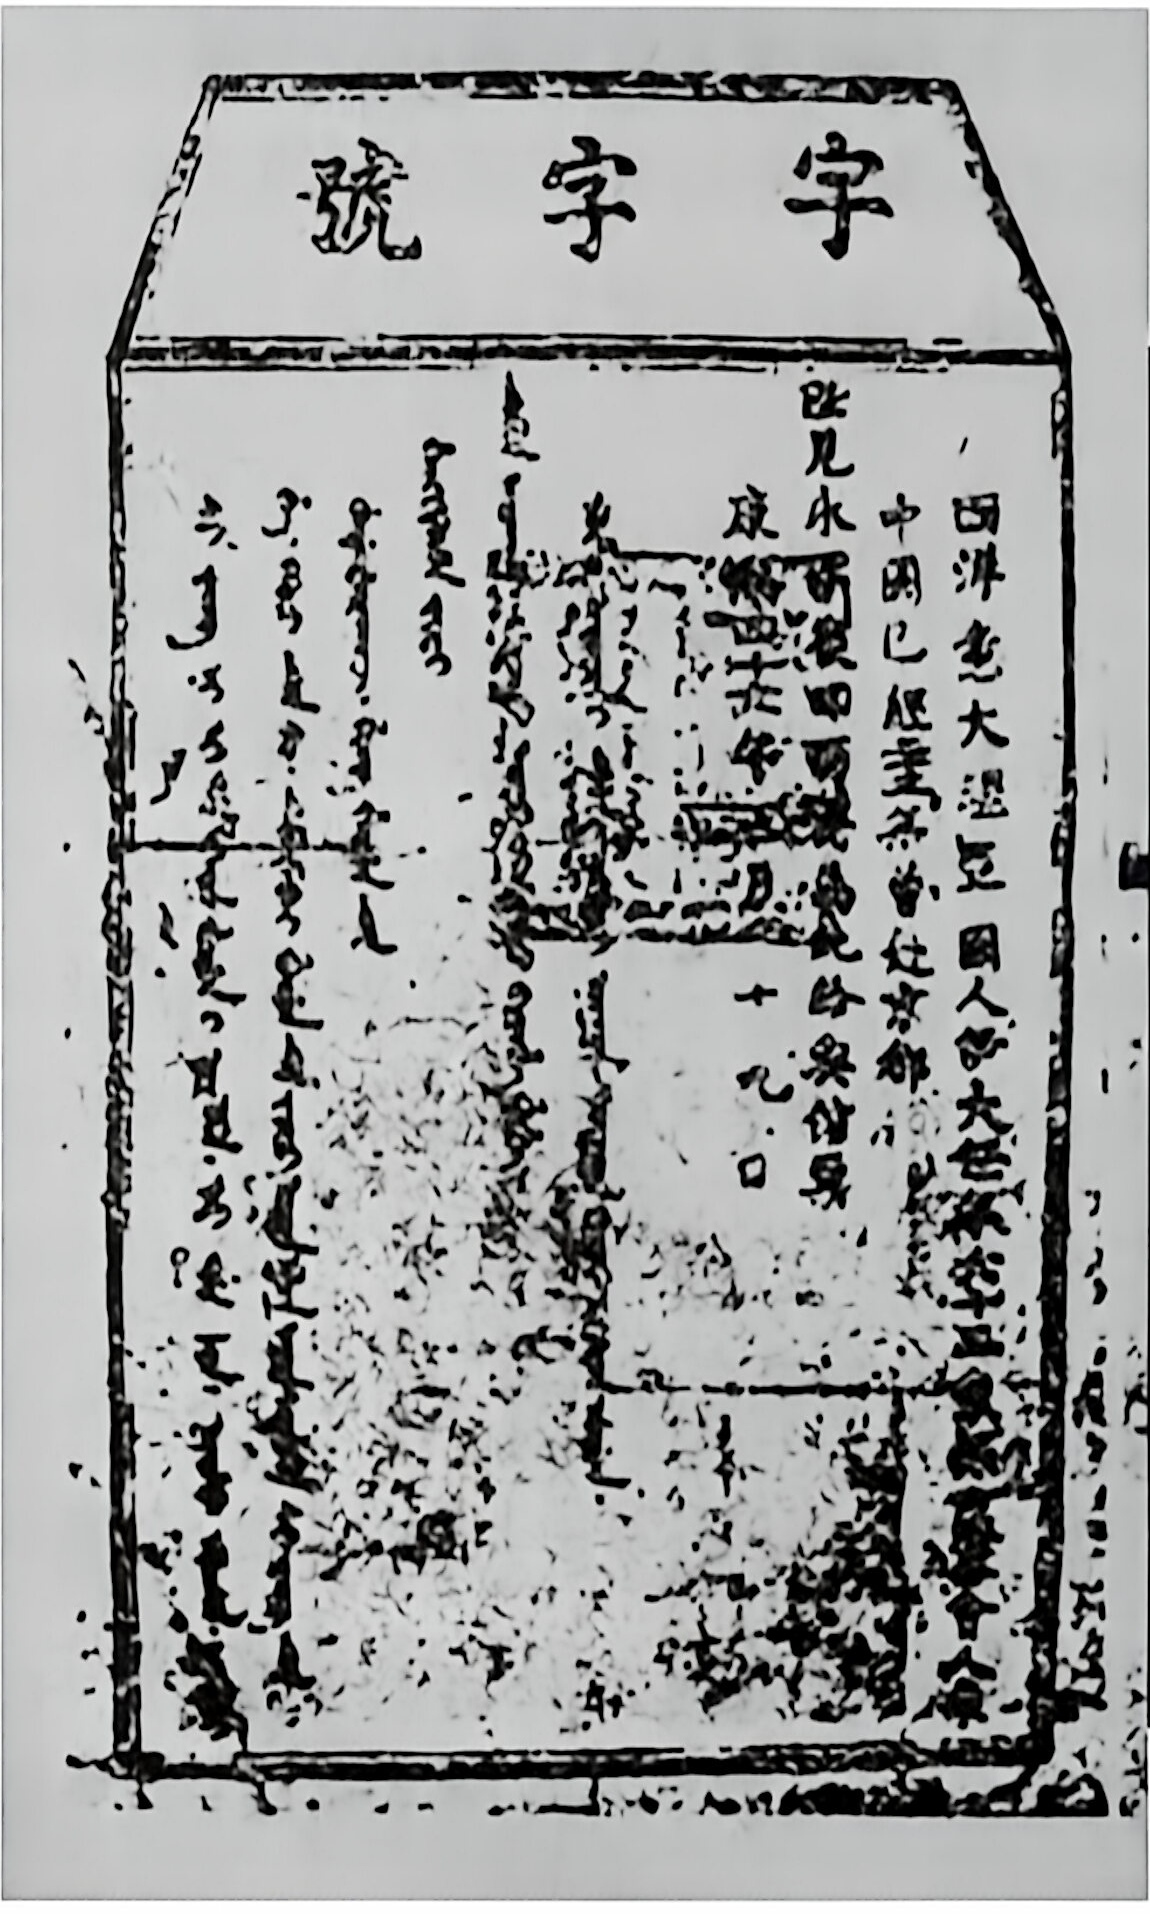
\includegraphics[width=\linewidth,height=.63\textheight,keepaspectratio]{assets/fig-36.jpg}
\caption{原印票}\end{subfigure}\hfill
\begin{subfigure}{.34\linewidth}\small\quotefont
西洋意大理亚国人伊大任年六十二岁方济格会人来中国已经二十二年曾赴京都陛见永不覆回西洋为此给与信票
\par\medskip
康熙四十六年正月十九日
\caption{印票释文}\end{subfigure}
\caption{内务府发给传教士的印票（鞠德源、田建一、丁琼，《清宫廷画家郎世宁》，34）}\label{fig:36}\end{figure}

% 原书第18页

后来，传教士在地方上出示印票时，由于地方官员从未见过内务府给僧侣发的身份文件，以为是假造的，便发信到他们认为应该管理传教士的礼部进行核实。康熙坚持传教士由内务府管理，让内务府把认证过的传教士名单知会礼部，再让礼部通过官僚机构的渠道知会各地官员。后来，再有相关传教士的问题，地方官员就直接发信到内务府问询。在这样来回的认证中，传教士在内务府中的地位也在官场中得到了确认，官员们都对他们礼让三分或者说敬而远之。有了这层身份的加持，自然如康熙所说，传教士“会无事平安”。最初康熙委派管理传教士印票事务的是大皇子。\NoteRef{01}{30}


% 原书第18页

传教士自己当然也知道能拿到内务府发放的印票，相当于是康熙的府中之人，属于康熙的私人圈子。纪理安为此在《北京纪事》中专门讲解过拿到印票后，他们与归礼部管理的和尚有了区别：


% 原书第19页

\begin{bookquote}那些说我们与和尚地位差不多的说法是不对的。和尚受官僚机构以及地方官的管辖。但我们拿的印票，不受制于任何官僚机构。而且就像赫世亨（注：康熙身边的包衣奴才）所说的那样，官员们看到我们的票后都会礼让三分。这些票都是皇上亲自发放的，又称“龙票”，上面有龙的标志，外加内务府总管的印。这样一来，有这个票的人就不受普通官员的管辖了。\end{bookquote}

% 原书第19页

\begin{bookquote}而且，欧洲人拿到的这个票是在皇帝御前发放的。这在中国来说是最高的待遇，象征着一种特别的恩宠。当然，这个票也不能拿出去胡乱使用，小心谨慎也是必不可少的。\NoteRef{01}{31}\end{bookquote}

% 原书第19页

纪理安用拉丁文写下这些，肯定有向罗马那边炫耀地位的意思。但了解清朝官僚运作机制以后，就明白他并没有夸张。内务府的人，属于康熙的私人圈子，在地方上他们确实不受地方官直接管辖。就算内务府的人在地方上犯了事，地方官员也要知会内务府，由内务府或者皇帝来处理。这种特权，就是纪理安所谓“不受制于任何官僚机构”的意思。


% 原书第19–20页

在康熙朝，北京总共有三间天主教的教堂：南堂（宣武门教堂）、东堂（王府井圣若瑟教堂）和北堂（1703年康熙赐地修建，原址位于蚕池口，光绪间迁至西什库）。因而在京传教士在康熙朝被统称为“三堂西洋人”。在康熙的整个人事布局中（包括其私人网络和朝廷系统），三堂西洋人与内廷养心殿、武英殿当差之人类似，都属于内廷奴才。他们的这一地位，在康熙六十大寿（1713）的庆贺盛典上也得以明确展示。当时各国使节、王公贵族、朝臣以及地方官和内廷的奴才仆从，都根据各自的身份站在不同的区域来向康熙祝寿行礼。而“三堂西洋人纪理安、苏霖、白晋、巴多明等”作为一队人被安排与内廷养心殿、武英殿当差之人等站在乾清门一侧参加仪式，并为康熙祝寿行礼，这个站位便说明了他们在当时整个朝堂之上的位置。\NoteRef{01}{32}只有理解了当时传教士的位置，特别是他们隶属于康熙的内务府，可以行走往来于康熙的内廷，才能理解为什么传教士能够记录连朝廷史官（正常情况下不能进入内廷）都记录不到的内廷之事。


\begin{sectionnotes}

% 原书注释：原书第390页
\BookNote{01}{18}{该地图的高精度图像见于美国国会图书馆：\url{https://www.loc.gov/} item/2010585650/。}

% 原书注释：原书第390页
\BookNote{01}{19}{对于是明军还是李自成军挖开的河堤，历史上存在争议。对这场洪水的最新跨学科研究参看M. Storozum, P. Lu, S. Wang et al. "Geoarchaeological Evidence of the AD 1642 Yellow River Flood That Destroyed Kaifeng, A Former Capital of Dynastic China"。}

% 原书注释：原书第390页
\BookNote{01}{20}{董少新，《浅谈全球史的史料问题：以明清鼎革史的西文原始史料为中心》，41。}

% 原书注释：原书第390页
\BookNote{01}{21}{汤开建，《沉与浮：明清鼎革变局中的欧洲传教士利类思与安文思》（上、下）；夏伯嘉，《从安文思与汤若望之间的恩怨论说明宫廷耶稣会士》。}

% 原书注释：原书第390页
\BookNote{01}{22}{Albert Chan, "A European Document on the Fall of the Ming Dynasty (1644–1649)", 105.}

% 原书注释：原书第390页
\BookNote{01}{23}{Irene Pih, Le Père Gabriel de Magalhães, Un jésuite portugais en Chine au XVIIe siècle, 94-95.}

% 原书注释：原书第391页
\BookNote{01}{24}{《清初西洋传教士满文档案译本》，266。}

% 原书注释：原书第391页
\BookNote{01}{25}{孙立天，《康熙的红票：全球化中的清朝》，第三章。}

% 原书注释：原书第391页
\BookNote{01}{26}{《平定三逆方略》，卷8，11b。}

% 原书注释：原书第391页
\BookNote{01}{27}{当时北京还有收编入八旗的俄罗斯人和他们的东正教教堂。这些人没有和天主教的人算在一起。刘小萌，《关于清代北京的俄罗斯人—八旗满洲俄罗斯佐领历史寻踪》。}

% 原书注释：原书第391页
\BookNote{01}{28}{AP1,406.}

% 原书注释：原书第391页
\BookNote{01}{29}{《清初西洋传教士满文档案译本》，311。}

% 原书注释：原书第391页
\BookNote{01}{30}{更多关于传教士身份的讨论，参看《康熙的红票》第四章“内务府的人”。内务府的研究，一直是清史中的热点，已经有众多有分量的专著问世。但传教士在内务府中的地位，是一个新的课题，未有过前人研究。现在笔者的研究得出的结论是传教士隶属于内务府，但到底他们归内务府下面哪一个部门管理，到底他们是否等同内务府中的喇嘛等许多更为细节的问题尚待进一步研究。}

% 原书注释：原书第391页
\BookNote{01}{31}{AP2,275.}

% 原书注释：原书第391页
\BookNote{01}{32}{《万寿盛典初集》，卷10，19a。对这次生日庆典的研究，参看陈葆真，《康熙皇帝的生日礼物与相关问题之探讨》。}

\end{sectionnotes}
\section{为什么会有《北京纪事》这部资料？}

% 原书第20–21页

首先需要明确的是，《北京纪事》写作的初衷并非专门记录北京官场之事，而是传教士用来记录教皇派到中国的第一位使节多罗（Charles-Thomas Maillard de Tournon）到达北京后各种事情的日志。《北京纪事》的记录开始于1705年12月，这是多罗即将到达北京的时刻。多罗在到达中国前，已经在印度停留了半年，在当地解决天主教在印度传播中的各种问题。北京的耶稣会传教士心里明白，多罗到中国主要是来解决传教士内部在中国礼仪问题上的相关争议。天主教是一个教规严密的宗教，在中国传教时，他们一些教规势必和中国习俗存在冲突。比如，中国传统士子要拜孔子，而天主教是一神教，不允许信徒祭拜其他偶像。有一些传教士认为天主教可以容纳拜孔子，因为孔子不是神，拜孔子只表示对孔子的尊重；但另一些传教士认为拜孔子时有祈祷成分，比如求孔子保佑科举成功等，这样就与一神教的教规发生了冲突。中国是传统的文明古国，习俗众多，如何对待，需要传教士在其内部进行界定。但天主教内部各派在许多问题的界定上不能达成一致。他们从明代晚期就开始争论，持续了五十年。\NoteRef{01}{33}1704年，经过数十年的调查取证，教皇终于决定要在天主教内部统一思想，对相关争论逐条做出裁决。简单来说，教皇的裁决与在北京的耶稣会传教士观点相悖，所以后者已经预感到教皇使节多罗入京后，会与他们发生争执。北京三个教堂的传教士在多罗还没有到达前就先开了会，在会上统一了思想，同时也决定要未雨绸缪，记录下多罗入华后的方方面面，如果以后与教皇使节在一些问题上产生分歧，他们好有凭据。他们推选出传教士纪理安来负责记录。


% 原书第21页

纪理安在《北京纪事》最开头的“致读者”部分，就明言：


% 原书第22页

\begin{bookquote}我知道欧洲将会出现各种对北京出使的记载。不过，我不会等到它们出现。我能做的就是把我的记录写出来。而且我写的每个字都是真实并有据可查的。\NoteRef{01}{34}\end{bookquote}

% 原书第22页

当时基本所有到过中国的欧洲使团在回到欧洲后，都有使团成员写下他们的中国见闻。北京传教士明白这一点，同时也知道多罗是由罗马传信部（Propaganda Fide）派出来的使节。北京传教士都是耶稣会成员，而传信部在罗马就与耶稣会关于如何在海外传教的议题存在分歧。更重要的是，北京的传教士并不打算服从多罗传过来的教皇旨意，并期待使节把他们的观点带回罗马。因而他们强烈感到有把双方的争论交流记录下来的必要，以免自身名誉受损。


% 原书第22–23页

纪理安出生在德国城市乌兹堡（Würzburg）。除了身为传教士外，他还在大学教授过数学，对化学也有研究。1695年纪理安入京后，康熙亲自面试了他，并让他负责在华建立一间皇家玻璃厂。\NoteRef{01}{35}该玻璃厂隶属于内务府，1696年建成，与北堂同处北京蚕池口。\NoteRef{01}{36}在纪理安的主持下，外加欧洲派有专门人员来传授技术，北京玻璃厂很快就达到了当时世界的顶尖水平。1706年，即建厂十年后到达中国的教皇使节，惊诧地发现，中国产的玻璃上添加的珐琅彩已经能与当时欧洲最有名的意大利威尼斯制品相提并论。\NoteRef{01}{37}也是因为忙于玻璃厂的事务，在《北京纪事》中可以看到纪理安对被派记录教皇使节活动这一额外且繁重的任务有一些抱怨。1711年后，康熙又委任他做了钦天监的监正。


% 原书第23页

在北京传教士里，纪理安还有个身份是公证员。传教士发回欧洲的文件，经他公证后，就相当于拥有官方认证。因此由他以公证员的角色来记录，也是对记录可靠性的保证。由于《北京纪事》最根本的目的是要向欧洲，特别是教廷显示出北京传教士的清白，也就是显示他们是在合理范围内、在不违背教义的情况下与教皇的使节多罗争论，因而《北京纪事》的产生过程十分严谨且规范。首先，纪理安写下他在北京的所见所闻，同时还以北京耶稣会的名义要求某些传教士来撰写他们亲自经历的事件。比如跟这本书有关的康熙废黜太子那次外出行猎途中的见闻，就是由跟随康熙出行的巴多明神父执笔的，纪理安将其直接放到了《北京纪事》中。纪理安每写完一部分，就会把稿件送到在开封的传教士骆保禄（Giampaolo Gozani）那里，由后者誊录一遍。这是因为纪理安字迹欠佳，而骆保禄是整个中国北方教区书写最工整漂亮的一位传教士。骆保禄抄写好的稿件，经过纪理安校对和稍加修改，再由其他北京传教士传阅，经多方审读后，方才确定下来。\NoteRef{01}{38}


% 原书第23–24页

可以想见，《北京纪事》最开始记录的时候，并没有计划持续很多年。但多罗入京后，天主教内部的礼仪问题把康熙本人也卷入到争论之中。本来多罗1706年就要离开中国，但在康熙的授意下，广东官员联系了澳门的葡萄牙人，把多罗软禁在澳门，直到他1710年去世。同时，康熙于1706年和1708年分别派了两组传教士作为他的钦差，到欧洲讲述他对礼仪之争的观点。由多罗入京引起的相关争论，并没有因其离开北京甚至去世而停止，《北京纪事》也在继续书写，直到1712年4月才停笔。


\begin{sectionnotes}

% 原书注释：原书第391页
\BookNote{01}{33}{关于中国礼仪之争的全过程，参看George Minamiki, The Chinese Rites Controversy from Its Beginning to Modern Times。新近总结: Ines G. Županov, and Pierre-Antoine Fabre, eds. The Rites Controversies in the Early Modern World.}

% 原书注释：原书第391页
\BookNote{01}{34}{AP1,4.}

% 原书注释：原书第391页
\BookNote{01}{35}{Benjamin A. Elman, On Their Own Terms: Science in China, 1550–1900, 208–209.}

% 原书注释：原书第392页
\BookNote{01}{36}{最新相关研究，参看薛吕，《清宫造办处玻璃厂、玻璃作名称及厂址考证》。}

% 原书注释：原书第392页
\BookNote{01}{37}{Emily Byrne Curtis, "Aspects of a Multi-Faceted Process: The Circulation of Enamel Wares between the Vatican and Kangxi's Court (1700–1722)", 48–49.}

% 原书注释：原书第392页
\BookNote{01}{38}{“introduction”,AP1,XVI-XVII.《北京纪事》第1卷开始前有84页的资料介绍（introduction）。本文有关该资料的各种信息均来自该介绍，以及 Claudia von Collani,“Kilian Stumpf and hisActa Pekinensia': Life, Context and Purpose of a Manuscript"。}

\end{sectionnotes}
\section{《北京纪事》为什么会记载北京宫廷之事？}

% 原书第24–25页

既然《北京纪事》是为记录与来华教皇使节的争论，那为什么又会详细记录了北京宫廷之事呢？其实这与当时北京传教士在京城中的特殊地位有关。如前所述，传教士由于与康熙母亲佟家的关系，在康熙铲除鳌拜前就已经进入到康熙的私人圈子。后来，传教士一直归康熙的内务府管理。就像康熙给教皇使节多罗讲到的那样，传教士是他“府内之人”。\NoteRef{01}{39}康熙接待多罗的各项事务，也都是内务府操办，同时康熙派遣的使节出使罗马，也是内务府在负责。因此，《北京纪事》中就会涉及康熙内务府的府中之事。也就是说，《北京纪事》中基本没有与朝廷大臣相关的朝中之事，却有一些当时康熙的家事。而太子废立所涉及的主要人物都是康熙的家里人，像大皇子、太子等，也是在接待多罗时经常出现的人物。


% 原书第25页

更具体的原因是在太子废立期间，传教士切实地被卷入其中。首先，在康熙废黜太子的那次围猎行程中，还有一件大事发生：康熙的皇十八子生病以至亡故。传教士被传召到行营中给皇十八子治病，因而他们近距离接触到了当时的康熙和太子。其次，康熙回京后，身体不适，屡次召传教士去给他诊病、送药。这使传教士有更多的机会进出内廷，因而留下了一些他们亲眼所见的记录。第三，就是徐日昇神父之死。除了料理丧事以外，康熙还传令北京传教士推选出接替徐日昇来负责与宫中联络的神父。传教士在这个推选过程中多次入宫，而这一时期康熙又正好和他的内阁为新太子人选发生多次争吵。比如传教士最后选好了接替徐日昇的人选，康熙却没能接见，因为他正在和大臣激烈争论新太子人选—当时众人要力推皇八子。没有见到康熙，传教士便和接待他们的康熙的包衣奴才聊起了争论的最新详情。


% 原书第25页

整体上说，当康熙在1706年介入到罗马教会内部关于礼仪问题的争论后，他就变成了这场争论的重要参与者。康熙个人的喜恶和看法对于北京的传教士如何处理礼仪争论来说越来越重要。正是这个原因，1706年后的《北京纪事》对康熙以及皇子的记录也增多了。当《北京纪事》记录到1708年秋第一次废黜太子之时，皇家相关的事就穿插记录在了各种教会事务之间。


\begin{sectionnotes}

% 原书注释：原书第392页
\BookNote{01}{39}{AP1, 112.}

\end{sectionnotes}
\section{为什么以前的学者没有使用《北京纪事》？}

% 原书第26页

《北京纪事》以拉丁文写成。写完后底本留在北京，抄本发回罗马。罗马的抄本全部完整地保存在罗马耶稣会档案馆中，文档编号是：Jap.Sin138。这套资料以前只有少数耶稣会学者使用过。而这套档案资料在很长时间内不被重视的一个主要原因，是教会有意识地杜绝其流传，因为这套资料里的核心出发点是要和教皇争论中国的礼仪问题，而教皇后来又数次重申他的观点。于是这套资料被雪藏了。这就使它和我们熟知的广为流传的许多耶稣会神父的信件拥有了不一样的历史轨迹。


% 原书第26页

教皇使节多罗到达北京后，也确实与北京传教士开始了各种大小事情的争论，执笔记录这些争论的纪理安神父事实上已经预感到这套资料将会在很长的时间内不见天日。他在最开头的“致读者”部分充满感情地写道：


% 原书第26–27页

\begin{bookquote}我为我当下正在卷入到的事感到悲伤。我一边在准备着把真实的一切传递给后人，又必须要同时准备迎接冷遇——就像要接受用篮子罩住我本已微弱的灯一样，把我写的历史永远地囚禁到档案室的围墙中。无论如何，我是写给永恒时光的。既然我写的都是真相，那么总有明智的读者会发现它的用处。这就够了。这比赞美本书作者更能让他为其付出而感到满足。赞美从来都不是他追求的。\end{bookquote}

% 原书第27页

纪理安确实预见到了这套资料的遭遇，果然一到罗马，它就被“囚禁到档案室的围墙中”了。好在2000年左右，也就是这套资料撰写大概三百年后，在澳门利氏学社的牵头下，世界各地耶稣会中擅长拉丁文的学者开始集体将这套资料译成英文。\NoteRef{01}{40}《北京纪事》有约1467手写页，最后由两位研究在华耶稣会历史的资深学者——澳大利亚的鲁保禄（Paul Rule，1937—2024）和德国的柯兰霓（Claudia von Collani） 联合校定编辑，从2015年起陆续出版。目前已经有三卷分别由两个出版社出版，分别是：


% 原书第27页

\begin{bookquote}第1卷，1705年12月—1706年8月：\end{bookquote}

% 原书第27页

\begin{bookquote}The Acta Pekinensia or Historical Records of the Maillard de Tournon Legation: First Transcribed Edition and English Annotated Translation, Volume I: December 1705-August 1706 Rome: Institutum Historicum Societatis Iesu, 2015, ISBN: 9788870412093.\end{bookquote}

% 原书第27页

\begin{bookquote}第2卷，1706年9月—1707年12月：\end{bookquote}

% 原书第27–28页

\begin{bookquote}The Acta Pekinensia or Historical Records of the Maillard de Tournon Legation, Volume II: September 1706-December 1707, Leiden: Brill, 2019, ISBN: 9789004396319\end{bookquote}

% 原书第28页

\begin{bookquote}第3卷，1708年1月—1709年2月：\end{bookquote}

% 原书第28页

\begin{bookquote}The Acta Pekinensia or Historical Records of the Maillard de Tournon Legation, Volume III: January 1708-February 1709, Leiden: Brill, 2024, ISBN: 9789004696884.\end{bookquote}

\begin{sectionnotes}

% 原书注释：原书第392页
\BookNote{01}{40}{关于这个项目最开始的介绍，见Paul Rule,“The Acta Pekinensia: A Key Source for the History of Christianity in China", 207–246。}

\end{sectionnotes}
\section{《北京纪事》的史料价值及其可信度}

% 原书第28页

从时间上看，《北京纪事》属于事件同时代人的记录。从内容上看，其信息来源有两种：一是亲身经历的所见所闻，二是打听来的消息。与本书康熙废立太子内容相关的记载，两种信息来源都有。应该说《北京纪事》中两种来源的记录都具有极高的可信度，根源在于当时北京传教士的特殊地位。比如本书前言开头所写康熙与太子见面的养心殿，就在内廷。这里没有特许，一般朝臣都不能进出。而纪理安当时整天出入的地方就在养心殿旁边。废立太子期间发生的一些事，是他们亲见亲闻的。这在本书后面的章节中将会细说。另一方面，由于传教士在内务府中的地位，他们获取信息的渠道都是北京权贵、宫中的太监或者康熙的包衣奴才，所以即便是他们打听来的信息，也有极高的价值。


% 原书第28–29页

《北京纪事》主要内容是写给欧洲人看的教会之事，又用拉丁文所记，因而纪理安落笔之时没有同时代清人的各种顾忌，可以做到理想中的“秉笔直书”。而且纪理安自己也明白历史事实与经过润饰的历史书写之间的差别，除了强调他所记载都有可靠的来源，他在“致读者”部分还做了说明：


% 原书第29页

\begin{bookquote}在皇帝那里当差已经让我很忙了，我根本不可能去琢磨另外一种历史（注：意思是经过修改的历史）。而且我都不知道我写的东西是否会永远处于黑暗中，我有什么必要还要去打磨它呢？\end{bookquote}

% 原书第29–30页

当然这是纪理安的主观申明，那么客观上到底《北京纪事》的可信度如何？纪理安笔下的北京宫廷斗争以及他对人和事的品评，并不是历史研究中经常提到的客观评价，而就是他心中主观想法的表达。但这种主观性其实正是真实性的体现。前面引用到的朱彝尊在听闻太子复立后，喜而赋诗。他主观的“喜”就是真情流露。纪理安在《北京纪事》中的文字也是如此。而朱彝尊和纪理安记录的可信度来自同一个客观事实：他们笔下的废黜太子相关记录是在不知道事件后续发展和结果的情况下写出来的。不知道后来的事，也就不存在众多历史材料被诟病的由“后见之明”带来的偏见。这一点是朱彝尊和纪理安的记录比后来知道事件结果总结出的历史，更加可信的原因。像康熙朝的《实录》是雍正登位后编撰出来的。就是没有看过《实录》的人，也能理解这是一本胜利者书写的历史，不可能存在对雍正不利的内容。


% 原书第30页

现存罗马的《北京纪事》原始抄本，分三次发回欧洲。第一批包括1705年12月到1707年10月的文档；第二批从1707年11月到1708年12月；第三批是1709年1月到1712年4月（缺失1709年9月到1711年9月的内容）。本书使用到的主要是第二批文档中的内容，特别是其中1708年秋到12月底的部分。在这批记录的最后（1708年12月底），有苏霖（José Soares）神父的确认函，确认他完整阅读并核实了到那年年底记录中的所有内容。这一部分在1709年初从北京发出，然后就保存在了罗马（第一批是1708年初送走；第三批1712年送出）。也就是说，本书用到的第二批材料是在纪理安不知道太子是否会复立，更不知道后来还有十几年的夺嫡之争的情况下书写出来的。除了太子以外，纪理安这段时期的记录中还提到过大皇子、皇三子、皇四子、皇八子以及皇十四子。他在写到这些皇子时，并不会因为后来夺嫡之争的结果，而影响到他对这些皇子的书写。这是这份记录最特殊的价值所在。因而，纪理安自己陈述中所说的，他写下的就是他看到、听到、想到的，并没有专门去“打磨”过，是可以相信的说法。

